\section{Results and discussion}\label{sec:results}

\subsection{Main comparison (E1)}
\Cref{tab:main} reports, for every regime and method, the number of seeds on which
the gradient tolerance was reached, together with median iterations, data passes,
wall time and test accuracy. Three observations stand out.

\emph{Reliability.} ASH-LR, Newton and Newton--CG converged on all $80$ problems.
Both gradient methods failed to reach the tolerance within 1,000 iterations on every
ill-conditioned regime (R2--R8), and L-BFGS failed on all seeds of R5, R6 and R8,
i.e.\ in the larger and the badly scaled problems. On raw Spambase (R8), the
unconverged gradient methods stopped at test accuracies of 0.44--0.56, against 0.91
for the converged solutions, which shows that non-convergence is not harmless.
Converged methods reached the same objective value up to a relative gap of about
$10^{-7}$, and their test accuracies differed by at most $0.002$ on the same seed.

\emph{Direct Newton is the fastest method.} With $d\le500$ dense features, forming
$X^\top DX$ is a single BLAS-3 operation, and Newton needed 4--13 iterations
everywhere. In wall time it was faster than every other method in every regime; in R4--R8 the
next fastest converged method was 2 to 240 times slower. In data passes it was also
the cheapest method except in R1 and R7, where L-BFGS was cheaper, and in R4, where
forming the $200\times200$ Hessian costs $d$ passes per iteration and Newton--CG used
fewer passes.

\emph{Among matrix-free methods, Newton--CG is more efficient than ASH-LR.}
ASH-LR required more passes than Newton--CG in every regime except R6, where the
two are statistically indistinguishable (\cref{tab:h1}). It was more efficient than
L-BFGS where L-BFGS struggled but converged (R3: median passes ratio 0.71 and five
times faster), and it converged where L-BFGS did not (R5, R6, R8).

\begin{table}[p]
\centering
\caption{E1: main comparison, $w_0=0$, $\lambda=10^{-6}$, tolerance
$\norm{g}\le10^{-6}$. Conv.\ = seeds converged out of ten; the other columns are
medians over the ten seeds. Passes are products with $X$ or $X^\top$.}\label{tab:main}
\footnotesize
\begin{tabular}{llrrrrr}
\toprule
Regime & Method & Conv. & Iter. & Passes & Time (ms) & Test acc. \\
\midrule
R1 & GD & 10/10 & 566 & 1,135 & 27.1 & 0.736 \\
 & GD-fixed & 10/10 & 136 & 273 & 6.2 & 0.736 \\
 & Newton & 10/10 & 4 & 50 & 0.6 & 0.736 \\
 & Newton-CG & 10/10 & 5 & 50 & 0.7 & 0.736 \\
 & L-BFGS & 10/10 & 16 & 34 & 1.4 & 0.736 \\
 & \textbf{ASH-LR} & 10/10 & 27 & 94 & 1.9 & 0.736 \\
\midrule
R2 & GD & 0/10 & 1000 & 2,002 & 49.4 & 0.746 \\
 & GD-fixed & 0/10 & 1000 & 2,002 & 44.9 & 0.754 \\
 & Newton & 10/10 & 4 & 50 & 0.6 & 0.746 \\
 & Newton-CG & 10/10 & 6 & 92 & 1.0 & 0.746 \\
 & L-BFGS & 10/10 & 60 & 128 & 5.2 & 0.746 \\
 & \textbf{ASH-LR} & 10/10 & 23 & 140 & 2.2 & 0.746 \\
\midrule
R3 & GD & 0/10 & 1000 & 2,002 & 59.8 & 0.738 \\
 & GD-fixed & 0/10 & 1000 & 2,002 & 54.9 & 0.736 \\
 & Newton & 10/10 & 4 & 50 & 0.8 & 0.742 \\
 & Newton-CG & 10/10 & 8 & 126 & 1.8 & 0.742 \\
 & L-BFGS & 10/10 & 192 & 416 & 25.5 & 0.742 \\
 & \textbf{ASH-LR} & 10/10 & 28 & 266 & 4.1 & 0.742 \\
\midrule
R4 & GD & 0/10 & 1000 & 2,002 & 554 & 0.722 \\
 & GD-fixed & 0/10 & 1000 & 2,002 & 534 & 0.725 \\
 & Newton & 10/10 & 5 & 1,034 & 36.9 & 0.721 \\
 & Newton-CG & 10/10 & 6 & 753 & 152 & 0.721 \\
 & L-BFGS & 10/10 & 467 & 952 & 299 & 0.720 \\
 & \textbf{ASH-LR} & 10/10 & 34 & 1,704 & 363 & 0.721 \\
\midrule
R5 & GD & 0/10 & 1000 & 2,002 & 1,557 & 0.717 \\
 & GD-fixed & 0/10 & 1000 & 2,002 & 1,693 & 0.716 \\
 & Newton & 10/10 & 5 & 2,605 & 265 & 0.705 \\
 & Newton-CG & 10/10 & 7 & 3,082 & 1,971 & 0.705 \\
 & L-BFGS & 0/10 & 1000 & 2,035 & 1,652 & 0.705 \\
 & \textbf{ASH-LR} & 10/10 & 37 & 6,990 & 4,645 & 0.705 \\
\midrule
R6 & GD & 0/10 & 1000 & 9,462 & 496 & 0.727 \\
 & GD-fixed & 0/10 & 1000 & 2,002 & 89.1 & 0.727 \\
 & Newton & 10/10 & 5 & 265 & 3.4 & 0.728 \\
 & Newton-CG & 10/10 & 492 & 46,162 & 828 & 0.728 \\
 & L-BFGS & 0/10 & 1000 & 2,086 & 153 & 0.725 \\
 & \textbf{ASH-LR} & 10/10 & 598 & 54,120 & 901 & 0.728 \\
\midrule
R7 & GD & 0/10 & 1000 & 2,002 & 236 & 0.920 \\
 & GD-fixed & 0/10 & 1000 & 2,002 & 239 & 0.920 \\
 & Newton & 10/10 & 10 & 595 & 16.0 & 0.921 \\
 & Newton-CG & 10/10 & 12 & 600 & 34.4 & 0.921 \\
 & L-BFGS & 10/10 & 142 & 294 & 49.7 & 0.921 \\
 & \textbf{ASH-LR} & 10/10 & 20 & 740 & 45.3 & 0.921 \\
\midrule
R8 & GD & 0/10 & 1000 & 16,906 & 2,379 & 0.564 \\
 & GD-fixed & 0/10 & 1000 & 2,002 & 250 & 0.441 \\
 & Newton & 10/10 & 13 & 773 & 19.3 & 0.909 \\
 & Newton-CG & 10/10 & 62 & 2,647 & 131 & 0.909 \\
 & L-BFGS & 0/10 & 1000 & 2,449 & 372 & 0.916 \\
 & \textbf{ASH-LR} & 10/10 & 76 & 3,122 & 180 & 0.909 \\
\bottomrule
\end{tabular}
\end{table}

\Cref{fig:conv} shows the relative objective gap against data passes for one seed in
four representative regimes. The curves make the cost structure of ASH-LR visible:
during the gradient phase (the first 15--40 passes) it tracks GD, and only after the
switch does it descend at the rate of a Newton-type method. In R2 and R5 the gradient
phase is pure overhead. In R6 and R8 ASH-LR and Newton--CG follow almost the same
path, with both needing hundreds of CG iterations per Newton step.

\begin{figure}[t]
\centering
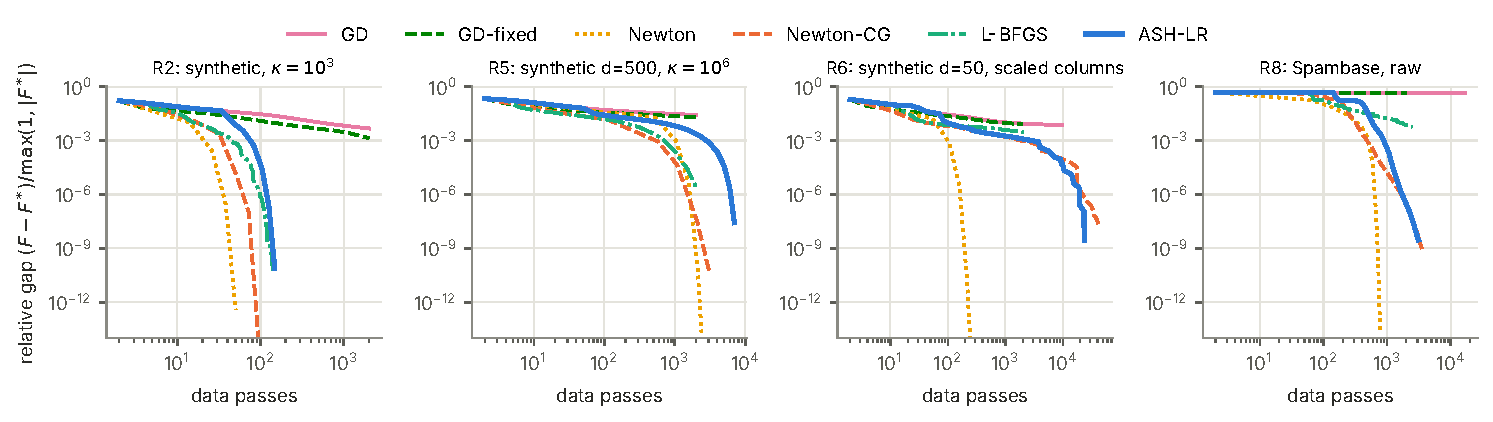
\includegraphics[width=\textwidth]{convergence_passes}
\caption{Relative objective gap versus data passes (seed 1000, log--log scale) in four
regimes. Direct Newton (dotted) reaches machine precision in a few hundred passes
in R6 and R8, where the matrix-free methods need tens of thousands.}\label{fig:conv}
\end{figure}

\subsection{Pre-registered hypothesis H1}
\Cref{tab:h1} gives, for the five primary regimes, the per-seed ratios of ASH-LR's
passes and times to those of each baseline that converged on all seeds. The best
converging matrix-free baseline was Newton--CG in all five regimes, and the change in
median passes of ASH-LR relative to it was $+111\%$ (R3), $+126\%$ (R4), $+127\%$
(R5), $+17\%$ (R6) and $+18\%$ (R8). ASH-LR therefore did not achieve the required
reduction of $20\%$ in any regime, and \textbf{H1 is not supported}. In R6 the
median per-seed ratio is $0.93$ and the Wilcoxon test does not detect a difference
($p=0.92$): ASH-LR was cheaper on some seeds and more expensive on others, and the
ratio of the medians ($1.17$) and the median of the ratios ($0.93$) point in
different directions, which itself indicates that the two methods are on a par there.

\begin{table}[t]
\centering
\caption{H1: per-seed ratios ASH-LR / baseline (median and interquartile range for
passes, median for time) and the two-sided Wilcoxon signed-rank $p$-value for passes
(ten seeds). Ratios below one favour ASH-LR. Baselines that did not converge on all
seeds are not compared.}\label{tab:h1}
\footnotesize
\begin{tabular}{llrrrr}
\toprule
Regime & Baseline & Conv. (base) & Passes ratio & Time ratio & $p$ (passes) \\
\midrule
R3 & Newton-CG & 10/10 & 2.03 [1.87, 2.56] & 2.31 & 0.002 \\
 & L-BFGS & 10/10 & 0.71 [0.54, 0.74] & 0.20 & 0.002 \\
 & Newton & 10/10 & 5.26 [4.79, 6.10] & 5.25 & 0.002 \\
\midrule
R4 & Newton-CG & 10/10 & 2.33 [1.99, 2.74] & 2.34 & 0.002 \\
 & L-BFGS & 10/10 & 1.80 [1.76, 2.08] & 1.21 & 0.002 \\
 & Newton & 10/10 & 1.65 [1.62, 1.92] & 9.51 & 0.002 \\
\midrule
R5 & Newton-CG & 10/10 & 2.25 [2.23, 2.30] & 2.26 & 0.002 \\
 & L-BFGS & 0/10 & \multicolumn{3}{c}{baseline not converged} \\
 & Newton & 10/10 & 2.68 [2.68, 2.70] & 16.92 & 0.002 \\
\midrule
R6 & Newton-CG & 10/10 & 0.93 [0.80, 1.30] & 0.85 & 0.922 \\
 & L-BFGS & 0/10 & \multicolumn{3}{c}{baseline not converged} \\
 & Newton & 10/10 & 204.40 [142.02, 238.40] & 252.76 & 0.002 \\
\midrule
R8 & Newton-CG & 10/10 & 1.17 [1.12, 1.31] & 1.28 & 0.014 \\
 & L-BFGS & 0/10 & \multicolumn{3}{c}{baseline not converged} \\
 & Newton & 10/10 & 4.15 [4.02, 4.45] & 9.02 & 0.002 \\
\bottomrule
\end{tabular}
\end{table}

\Cref{fig:ratios} extends the comparison to all regimes. ASH-LR uses between about
1.2 and 2.3 times the passes of Newton--CG, except in R6, and the ratio to direct
Newton grows to two orders of magnitude in the badly scaled synthetic regime.

\begin{figure}[t]
\centering
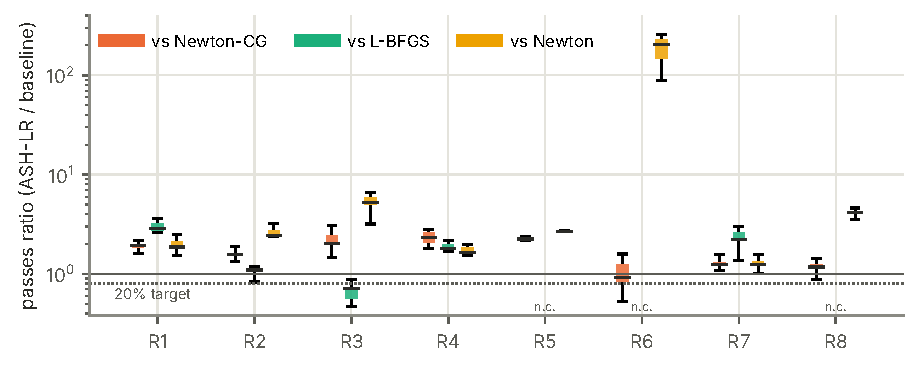
\includegraphics[width=0.85\textwidth]{ratios}
\caption{Ratio of data passes, ASH-LR over each baseline, across the ten seeds of
every regime (boxes: interquartile range; line: median). Values below the solid line
favour ASH-LR; the dotted line marks the 20\% target. ``n.c.'': baseline not converged
on all seeds.}\label{fig:ratios}
\end{figure}

\subsection{Ablation (E3)}
\Cref{tab:ablation} isolates the components of ASH-LR, and \cref{fig:ablation}
displays the median passes.

\begin{table}[t]
\centering
\caption{E3: ablation of ASH-LR (ten seeds, $w_0=0$). Conv.\ = seeds converged;
Passes = median data passes. (a) is the Milestone~2 method and (d) the final method.}\label{tab:ablation}
\footnotesize
\begin{tabular}{lrrrrrrrr}
\toprule
Variant & \multicolumn{2}{c}{R2} & \multicolumn{2}{c}{R5} & \multicolumn{2}{c}{R6} & \multicolumn{2}{c}{R8} \\
 & Conv. & Passes & Conv. & Passes & Conv. & Passes & Conv. & Passes \\
\midrule
(a) M2: direct+LS, fixed $\mu$ & 10/10 & 118 & 10/10 & 6,817 & 10/10 & 749 & 10/10 & 942 \\
(b) CG+LS, fixed $\mu$ & 10/10 & 168 & 10/10 & 6,541 & 10/10 & 48,208 & 10/10 & 2,796 \\
(c) CG+ratio, fixed $\mu$ & 10/10 & 168 & 10/10 & 6,541 & 10/10 & 48,208 & 10/10 & 3,033 \\
(d) ASH-LR (full) & 10/10 & 140 & 10/10 & 6,990 & 10/10 & 54,120 & 10/10 & 3,122 \\
(e) full, no GD phase & 10/10 & 91 & 10/10 & 5,686 & 10/10 & 39,316 & 10/10 & 3,192 \\
(f) direct+ratio, grad $\mu$ & 10/10 & 105 & 10/10 & 6,817 & 10/10 & 644 & 10/10 & 912 \\
\bottomrule
\end{tabular}
\end{table}

\begin{figure}[t]
\centering
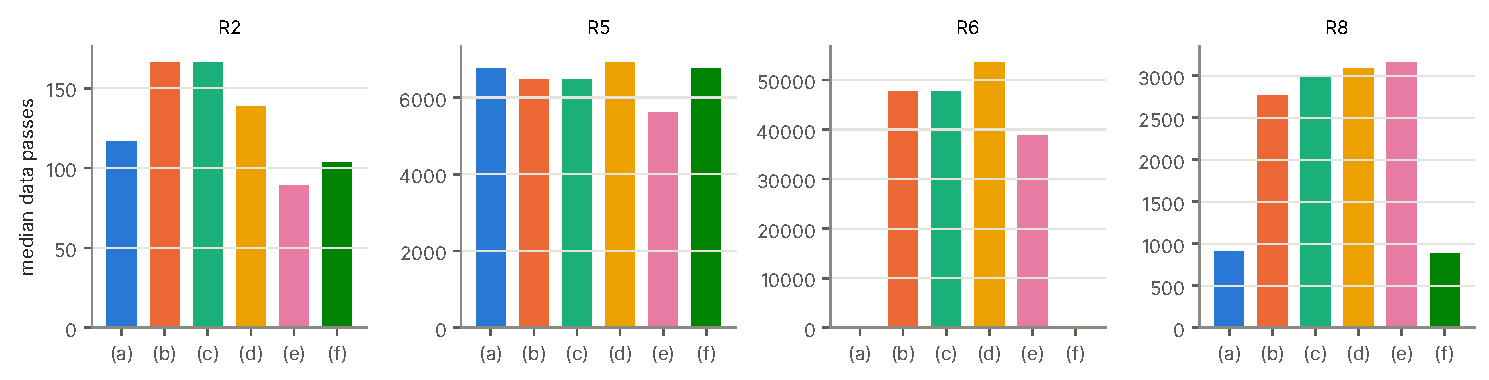
\includegraphics[width=\textwidth]{ablation}
\caption{E3: median data passes of the six ASH-LR variants.}\label{fig:ablation}
\end{figure}

\paragraph{The gradient phase is the main overhead} Removing it (variant e) reduced
the median passes in R2, R5 and R6 (by 35\%, 19\% and 27\%) and, in R2 and R5,
cut the number of iterations by roughly 70\%. Only on raw Spambase did it help slightly (3,121 vs.
3,193 passes). Because Newton's method on the logistic loss is well behaved from
$w_0=0$, as also observed for truncated Newton methods on linear
classification~\cite{galli2022truncated}, the
cautious start that motivated the gradient phase is rarely needed. This finding is
post hoc: the final method was frozen with the gradient phase, as specified.

\paragraph{The inner solver dominates in badly scaled problems} In R6 and R8 the dense-solve
variants (a) and (f) needed only 16--21 iterations, whereas every CG variant needed
434--598 iterations in R6 and 67--80 in R8. The cause is the inexact
solve: with a Hessian condition number around $10^{8}$--$10^{9}$ at the start
(\cref{tab:regimes}), unpreconditioned CG cannot reduce the residual by the forcing
factor within $d$ iterations, so the Newton steps are poor and many of them are
needed. Damping cannot repair this: in R8 the ratio test rejected a median of 18
trial steps per run, and the trace in \cref{fig:trace} shows $\mu$ jumping to about
$20$ after a series of rejections before it decays geometrically with the
gradient norm.

\paragraph{Damping rules} The gradient-regularized rule helped when combined with an
exact solve (f vs.\ a: 11\%, 14\% and 3\% fewer passes in R2, R6 and R8). With CG, it
was slightly worse than the fixed rule in R5, R6 and R8 (d vs.\ c), because a larger
$\mu$ early in the Newton phase makes the CG systems easier but the steps shorter.
Variants (b) and (c) produced identical iterates in R2, R5 and R6: when every trial
step is accepted with $\rho>0.75$, the ratio test and the line-search rule both
halve $\mu$, so the two rules only differ on problems with rejected steps.

\begin{figure}[t]
\centering
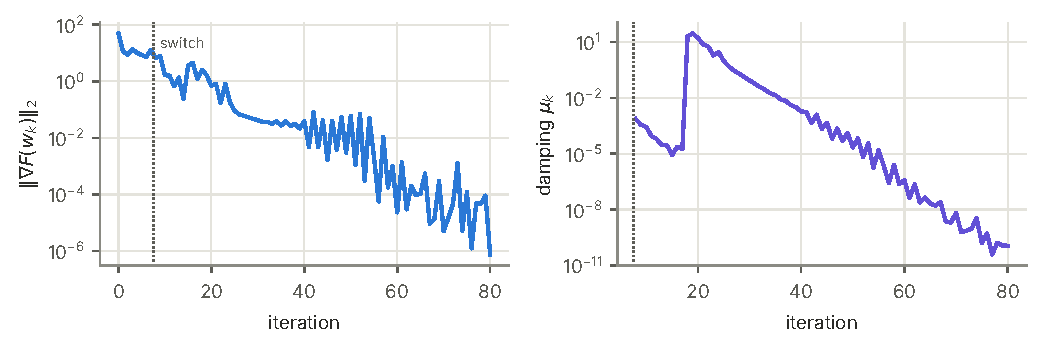
\includegraphics[width=0.85\textwidth]{trace_R8}
\caption{ASH-LR on R8 (seed 1000): gradient norm and damping per iteration. The
dotted line marks the switch to the Newton phase.}\label{fig:trace}
\end{figure}

\subsection{Robustness to starting point and regularization (E2)}
\Cref{tab:robust} summarizes 81 problems per method (three regimes, three seeds,
three values of $\lambda$, three starting points). ASH-LR, Newton and Newton--CG
converged on all 81 problems, never produced a non-finite value and never failed a
line search. L-BFGS converged on 47 of 81; it failed on 25 of the 27 raw-Spambase
problems and on all nine R5 problems with $\lambda=10^{-6}$. Robustness is thus shared by all three Newton-type
methods and is not a distinguishing advantage of ASH-LR. A distant start hurt
ASH-LR most: on R2 its median work grew from 122 passes ($w_0=0$) to 1,080 (far
start), because with saturated logits the gradient is small and the switching rule
keeps the method in the slow gradient phase for longer. Newton--CG grew only from
88 to 132 passes. Larger $\lambda$ improves the conditioning and reduced the work of
all methods; for $\lambda=10^{-2}$ Newton--CG needed a median of 86 passes against
380 for ASH-LR.

\begin{table}[t]
\centering
\caption{E2: seeds converged and, in parentheses, median data passes over the three
seeds and three values of $\lambda\in\{10^{-6},10^{-4},10^{-2}\}$ (nine problems per
cell). Relative stopping rule $\norm{g}/\max(1,\norm{g_0})\le10^{-6}$.}\label{tab:robust}
\footnotesize
\begin{tabular}{llrrrr}
\toprule
Regime & Start & Newton & Newton-CG & L-BFGS & ASH-LR \\
\midrule
R2 & zero & 9/9 (50) & 9/9 (88) & 9/9 (111) & 9/9 (122) \\
 & near & 9/9 (64) & 9/9 (90) & 9/9 (99) & 9/9 (192) \\
 & far & 9/9 (96) & 9/9 (132) & 9/9 (141) & 9/9 (1,080) \\
\midrule
R5 & zero & 9/9 (2,084) & 9/9 (518) & 6/9 (426) & 9/9 (802) \\
 & near & 9/9 (3,127) & 9/9 (532) & 6/9 (470) & 9/9 (1,050) \\
 & far & 9/9 (3,662) & 9/9 (686) & 6/9 (530) & 9/9 (1,990) \\
\midrule
R8 & zero & 9/9 (595) & 9/9 (456) & 0/9 (2,508) & 9/9 (1,040) \\
 & near & 9/9 (657) & 9/9 (584) & 1/9 (2,469) & 9/9 (866) \\
 & far & 9/9 (921) & 9/9 (471) & 1/9 (2,449) & 9/9 (805) \\
\bottomrule
\end{tabular}
\end{table}

\subsection{Single precision (E4) and numerical stability (E5)}
In single precision with tolerance $10^{-4}$ (\cref{tab:f32}), all three methods
converged on R2 and standardized Spambase (R7), with objective gaps comparable to
double precision and wall times 4--55\% lower. On raw Spambase (R8), however,
Newton--CG converged on none and ASH-LR on one of three seeds, while direct Newton
converged on all. With a Hessian condition number near $10^{9}$, which exceeds
$1/\epsilon_{\text{float32}}\approx1.7\times10^{7}$, the rounding errors in the
Hessian-vector products and CG recurrences~\cite{higham2022mixed} are large enough to make the inexact
Newton steps unreliable, whereas the dense factorization still delivers usable
steps. Single precision is therefore safe only for reasonably scaled data when the
inner solver is CG.

\begin{table}[t]
\centering
\caption{E4: float64 versus float32 (tolerance $10^{-4}$, three seeds). Median
relative gap of the returned solution evaluated in float64, and ratio of median wall
times.}\label{tab:f32}
\footnotesize
\begin{tabular}{llrrrrr}
\toprule
Regime & Method & \multicolumn{2}{c}{Conv.} & \multicolumn{2}{c}{Median gap} & Time ratio \\
 & & f64 & f32 & f64 & f32 & f32/f64 \\
\midrule
R2 & Newton & 3/3 & 3/3 & 2.1e-13 & 2.4e-13 & 0.79 \\
 & Newton-CG & 3/3 & 3/3 & 1.2e-08 & 1.1e-06 & 0.93 \\
 & ASH-LR & 3/3 & 3/3 & 7.8e-07 & 8.9e-07 & 0.96 \\
\midrule
R7 & Newton & 3/3 & 3/3 & 2.7e-09 & 2.8e-09 & 0.57 \\
 & Newton-CG & 3/3 & 3/3 & 1.9e-07 & 2.4e-07 & 0.45 \\
 & ASH-LR & 3/3 & 3/3 & 1.1e-05 & 3.2e-07 & 0.53 \\
\midrule
R8 & Newton & 3/3 & 3/3 & 1.0e-10 & 1.0e-10 & 0.58 \\
 & Newton-CG & 3/3 & 0/3 & 1.8e-05 & 5.9e-05 & 29.38 \\
 & ASH-LR & 3/3 & 1/3 & 3.3e-05 & 3.0e-05 & 37.60 \\
\bottomrule
\end{tabular}
\end{table}

\Cref{tab:stab} reports the stability test from an extreme starting point (logit
standard deviation $10^3$). With the stable formulas both methods converged on every
problem in double precision. With the naive formulas the initial loss overflows to
$+\infty$; every subsequent trial point whose margins still exceed the overflow
threshold also evaluates to $+\infty$, so line searches and ratio tests cannot
compare candidates. ASH-LR failed in all twelve naive runs, and Newton recovered in
only three of the six double-precision runs, when its first full step happened to
land at finite values. In single precision, where $\exp$ overflows already beyond
$|z|\approx88$, all naive runs failed. The only failures with the stable formulas
were the ASH-LR runs on R8 in float32, which reached the iteration limit with finite
values, consistent with the CG precision issue above. Stable evaluation is cheap and
exact, and it is the one component of ASH-LR whose benefit is unconditional.

\begin{table}[t]
\centering
\caption{E5: seeds converged out of three from an extreme start (logit standard
deviation $10^3$) with stable and naive formulas.}\label{tab:stab}
\footnotesize
\begin{tabular}{lllrrl}
\toprule
Regime & Precision & Formulas & Newton & ASH-LR & Failure mode \\
\midrule
R2 & float64 & stable & 3/3 & 3/3 & -- \\
 & float64 & naive & 2/3 & 0/3 & non finite \\
 & float32 & stable & 3/3 & 3/3 & -- \\
 & float32 & naive & 0/3 & 0/3 & non finite \\
\midrule
R8 & float64 & stable & 3/3 & 3/3 & -- \\
 & float64 & naive & 1/3 & 0/3 & non finite \\
 & float32 & stable & 3/3 & 0/3 & max iter \\
 & float32 & naive & 0/3 & 0/3 & non finite \\
\bottomrule
\end{tabular}
\end{table}

\subsection{Discussion}
The results give a consistent picture of when the ideas behind ASH-LR pay off.

\emph{Stable evaluation} is necessary, not optional: it costs nothing, changes no
iterate when the naive formulas are finite, and prevents total failure from distant
starting points or in single precision.

\emph{Second-order information} is what makes ill-conditioned logistic regression
tractable: all Newton-type methods converged everywhere, while first-order methods
and, on badly scaled data, L-BFGS did not. This supports the premise of the project.

\emph{The hybrid structure} did not pay off in our regimes. The gradient phase costs
15--40 passes that Newton-type methods do not need from $w_0=0$, and it becomes
expensive from distant starts. The damping mechanism worked as designed---$\mu$
grew after rejected steps and vanished near the solution---but with CG as the inner
solver the bottleneck in badly scaled problems is the accuracy of the inner solve,
which damping cannot fix. A diagonal (Jacobi) or randomized Nystr\"om
preconditioner~\cite{frangella2023randomized}, or simply feature scaling, would
attack the actual cause; the dramatic difference between R7 and R8, which differ
only by standardization, makes the same point from the data side.

\emph{Passes versus time.} For $d\le500$ dense features, the BLAS-3 Hessian
formation of direct Newton runs so much faster per flop than the matrix--vector
products of CG that direct Newton wins in time even where it loses in passes (R4).
Matrix-free methods become necessary only when $d$ is so large that $d^2$ memory or
$d^3$ work is prohibitive, or when $X$ is sparse; our experiments do not cover that
regime, so they cannot show whether ASH-LR would then compete with Newton--CG.

\paragraph{Threats to validity} Timings come from one virtual machine with two cores
and three repetitions; passes, which are machine-independent, lead to the same
conclusions. The synthetic designs have log-spaced spectra and logistic labels and
may be easier or harder than real data. Spambase contains 391 duplicate rows, which
affects test accuracy but not the optimization comparison. Finally, the ASH-LR
parameters (switching thresholds, $\mu_0$, update factors) were not tuned. The
ablation bounds what tuning the switch could achieve: even with no gradient phase at
all (variant e), ASH-LR matched Newton--CG in R2 (91 vs.\ 92 passes), used 15\%
fewer passes in R6 (39,316 vs.\ 46,162), and stayed behind in R5 and R8. This
post-hoc observation suggests that a damped Newton--CG without the gradient phase may
be competitive on badly scaled problems, but it would need its own pre-registered
test.

